
\item A particle A moves along a circle of radius \( R = 50 \) cm so that its radius vector \( \mathbf{r} \) relative to the point \( O \) (Fig. 1.5) rotates with the constant angular velocity \( \omega = 0.40 \) rad/s. Find the modulus of the velocity of the particle, and the modulus and direction of its total acceleration.
    \begin{center}
        % Since the image of the diagram is not provided, a placeholder is used here
        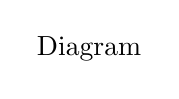
\begin{tikzpicture}
            \node at (0, 0) {Diagram}; % Replace this with the actual diagram or remove if not necessary
        \end{tikzpicture}
    \end{center}
    % If there are any subquestions, they would be added here. 
    % Given that there are no subquestions in the provided text, the enumerate environment is not used.

\begin{solution}
    \begin{center}
        \begin{tikzpicture}
            \pic at (0, 0) {frame=3cm};
        \end{tikzpicture}
    \end{center}
    
    \begin{align*}
        \intertext{Angular velocity of point \( A \), with respect to centre \( C \) of the circle or turning rate of line \( CA \) taking the line \( OCX \) as reference line becomes}
        \omega_C &= -\dfrac{d(2\theta)}{dt} = 2\left(-\dfrac{d\theta}{dt}\right) = 2\omega
        \intertext{because angular speed of line \( OA \) is \(\omega = -d\theta/dt\).} 
        \intertext{The turning rate of line \( CA \) is also the turning rate of velocity vector of point \( A \), which is given by \( v_A/R \).}
        \intertext{So, \( v_A = \omega_C R = (2\omega) R = 0.4 \, \text{m/s} \) (on substituting values).}
        \intertext{Alternate:}
        \intertext{Angular speed of a point relative to origin is }
        \omega &= \dfrac{\text{transverse velocity}}{\text{magnitude of position vector}}
        \intertext{So, angular speed of point \( A \) relative to origin \( O \) }
        \omega &= \dfrac{\text{component velocity of point A perpendicular to \( OA \)}}{\text{Length of line \( OA \)}}
        \omega &= \dfrac{v_A \cos \theta}{r}
        \intertext{But from sine property of triangle \( OAC \), \( r = 2R \cos \theta \).}
        \omega &= \dfrac{v_A}{2R} \quad \text{or} \quad v_A = 2\omega R
        \intertext{From both methods the obtained speed \( v_A \) is constant, so the tangential acceleration of particle \( A \) is zero and}
        w &= w_n = \dfrac{v_A^2}{R} = \dfrac{(2\omega R)^2}{R} = 4\omega^2 R = 0.32 \, \text{m/s}^2 \, \text{(on substituting values)}
    \end{align*}
\end{solution}

